\chapter{Appendix A}

One of the most interesting aspect of the work presented in this thesis is the manner in which it has been reached. Starting from now I want to clarify that during the first days it was not easy to understand the real objective of our work. Because of this initial misunderstanding we implemented some both strange and wrong solutions. Even if some of these solutions were not useful for the objective described in this thesis, they were very efficient in other context. For this reason we will here recall all the history of the work. We identify ten different main steps. 

\paragraph{First Step} In the first attempt to reach the solution of the problem we allowed the agent to make five different actions :

\begin{itemize}
	\item Move North
	\item Move South
	\item Move West
	\item Move East
	\item Dig
\end{itemize}

It is clear that we distinguished between the possibility for the agent to make a \textit{movement action} and a \textit{dig action}. In this choice we were inspired from the possibility of the human to make movement without doing nothing. We later understood that this implementation was absolutely redundant. Humans move themselves without doing nothing before decide to do something. A RL agent \textit{decide} what to do in the next step immediately after have finished the previous action without needing \textit{time to think}. \\

In this step the state was represented by three elements :

\begin{itemize}
	\item Coordinate $x$;
	\item Coordinate $y$;
	\item Number of remaining function soundings.
\end{itemize}

As already mentioned, such a state representation prevents from the possibility to generalize the training. Given two different bivariate functions $f(x, y)$ and $g(x, y)$ and supposing to have trained the RL agent using function $f(x, y)$ if we decide to sound $g(x, y)$ on point $x$ and $y$ already sounded in $f(x, y)$ the result will be completely different (see figures ~\ref{fig:2xy} and ~\ref{fig:xsin(y)} ). In addition to this the number of remaining function soundings is redundant and it does not add any information to our knowledge.

\begin{figure} [h!]
	\centering
	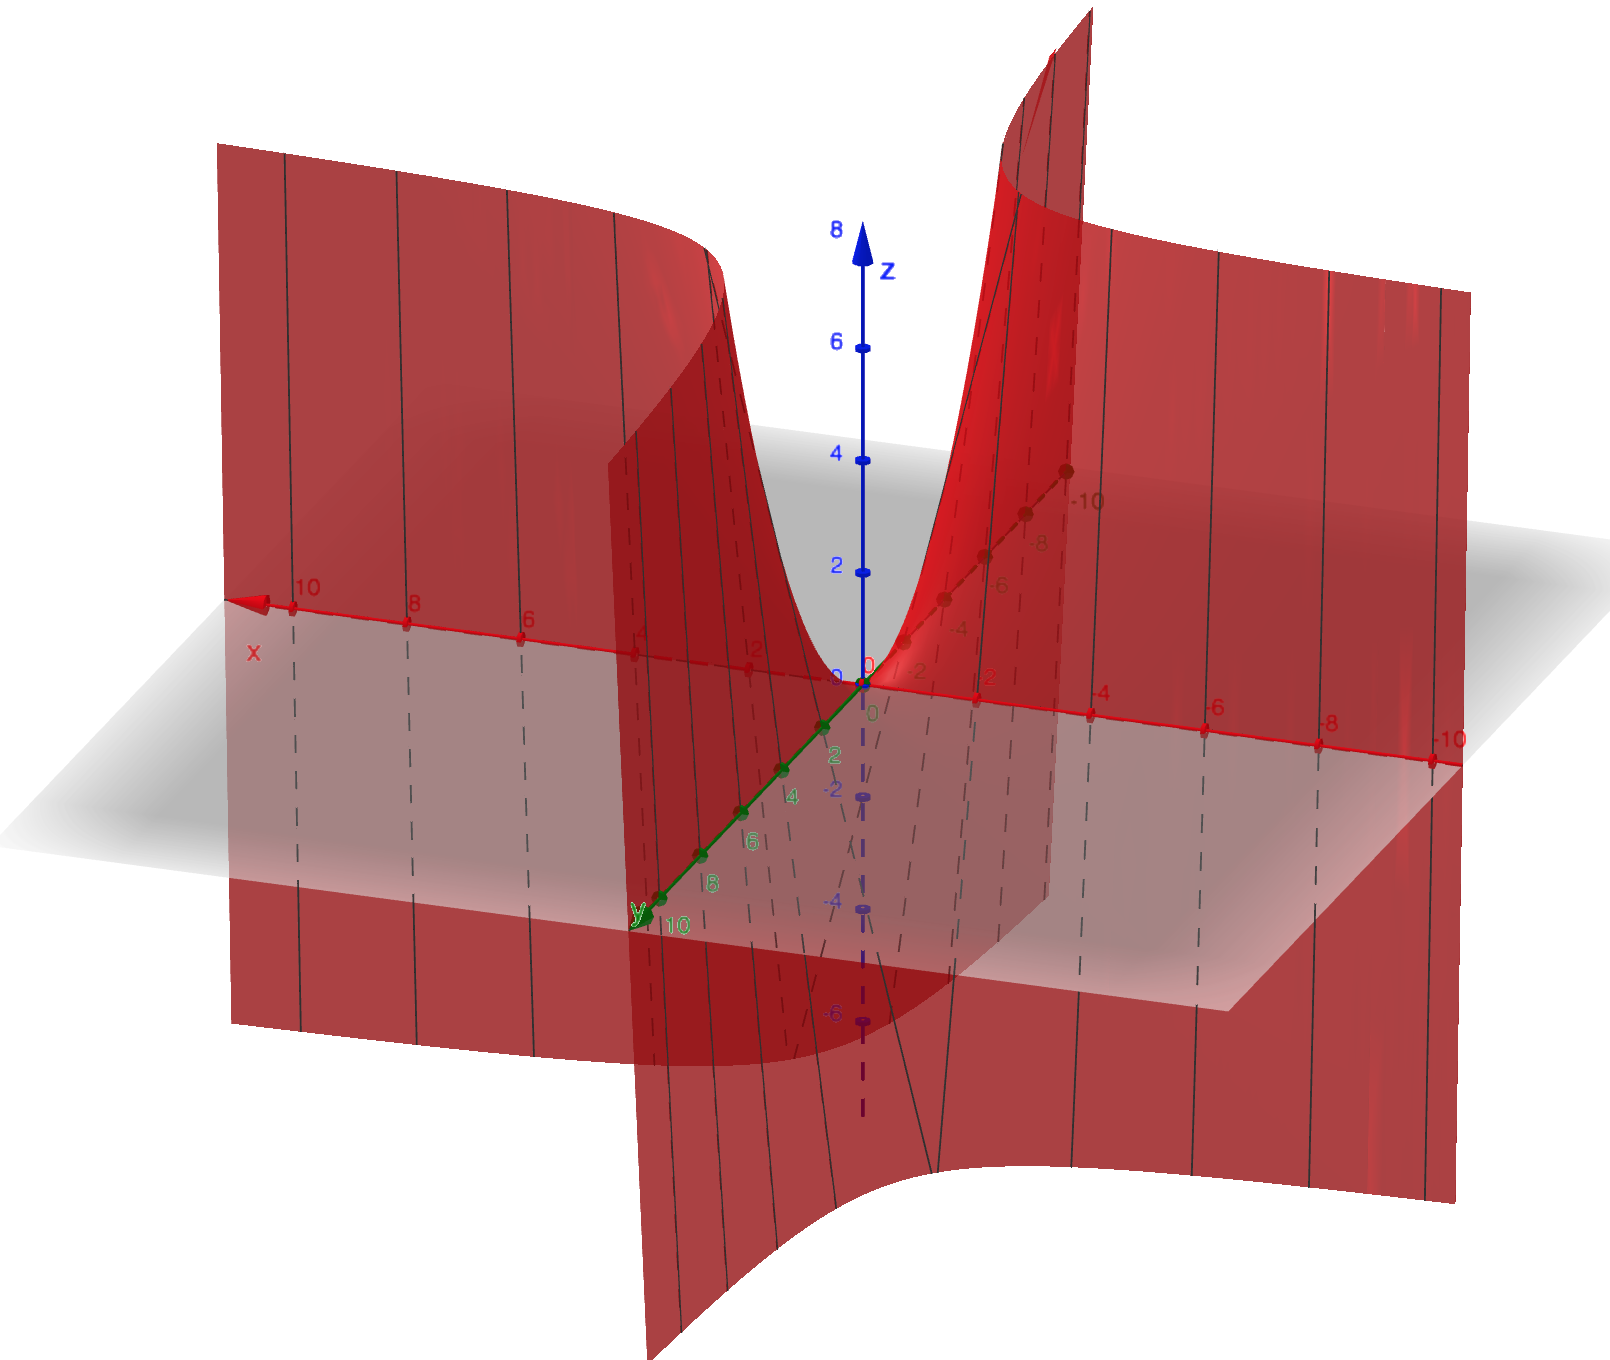
\includegraphics[width= 8cm, height = 9cm]{2xy}
	\caption{$f(x, y) = 2xy$, \quad $f(1, 1) = 2$}
	\label{fig:2xy}
\end{figure}

\begin{figure} [h!]
	\centering
	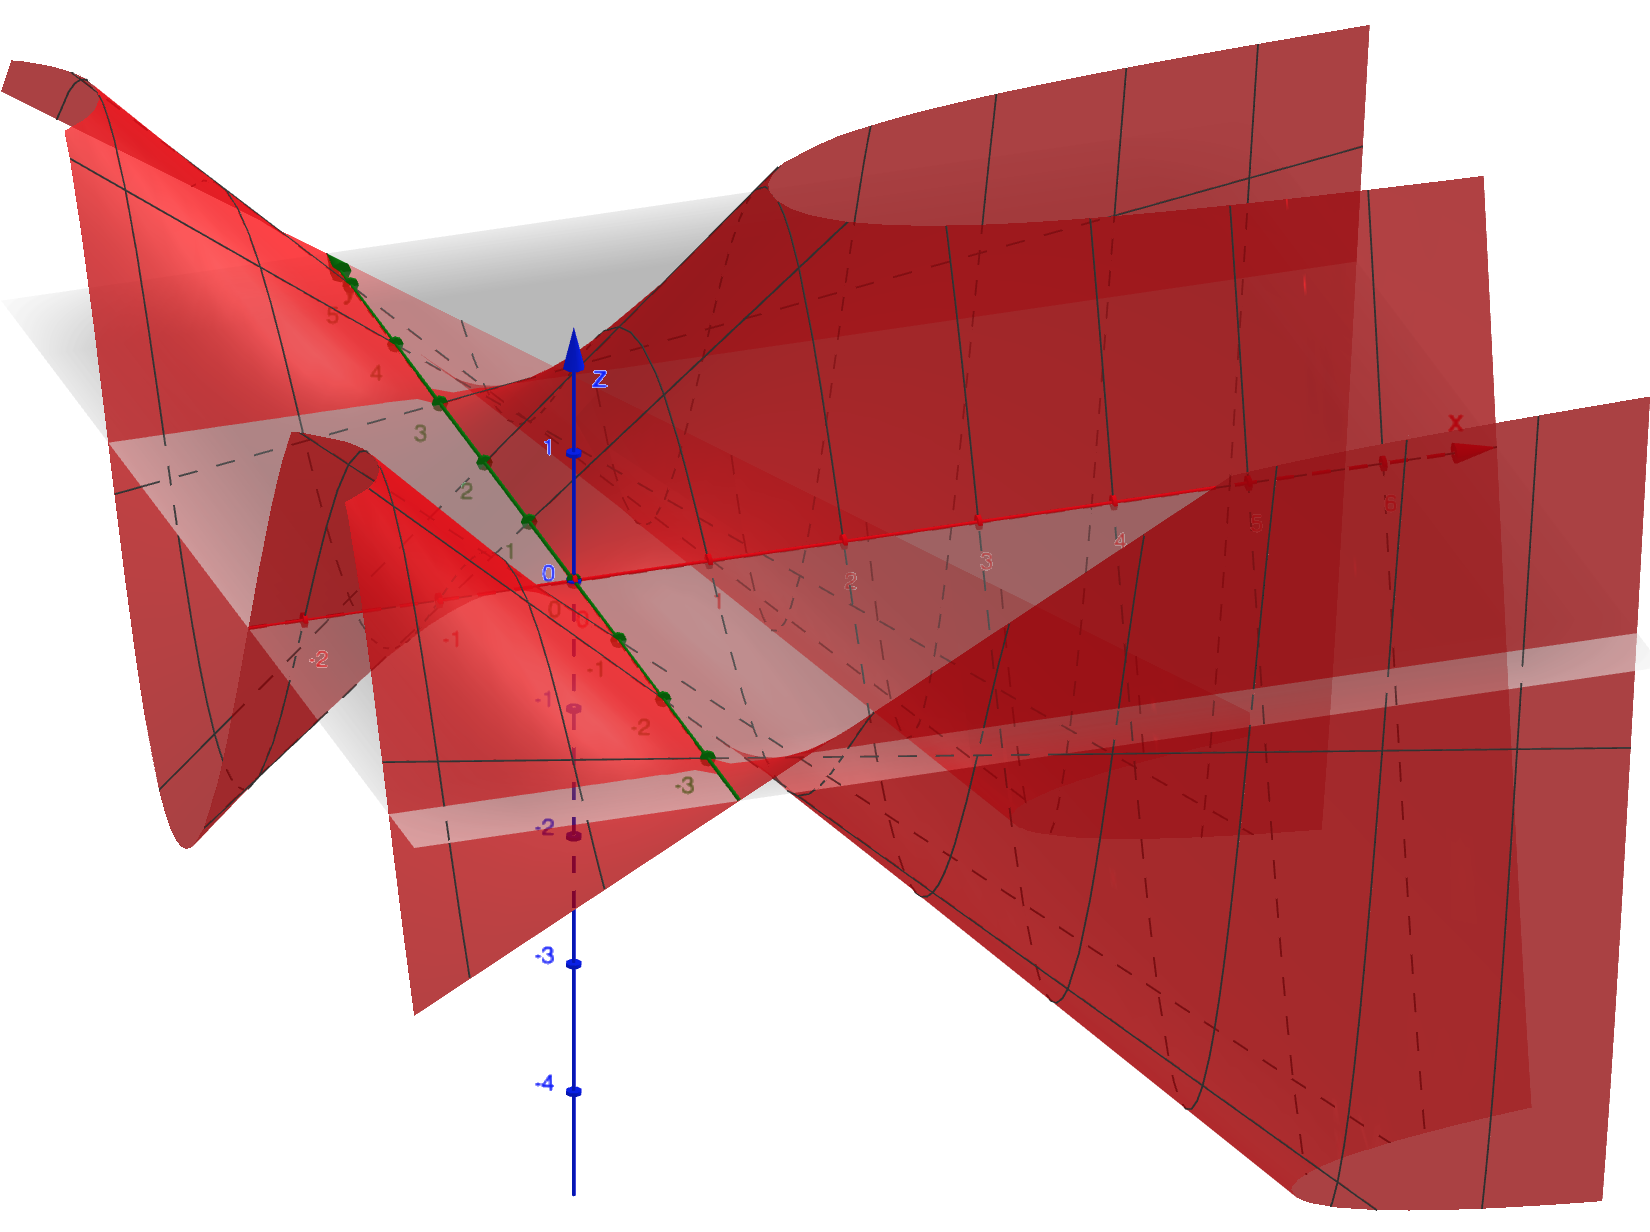
\includegraphics[width= 8cm, height = 9cm]{xsin(y)}
	\caption{$g(x, y) = x*sin(y)$, \quad $g(1, 1) = 0.017$}
	\label{fig:xsin(y)}
\end{figure} 

In this first step the reward was computed as the value of the function computed in $x$ and $y$ at time \textit{t}. The agent is in a terminal state when the number of remaining function soundings is equal to zero.

\paragraph{Second Step} The second step is globally equals to the first one except for two fundamental aspects. In this step we introduced the possibility for the agent to make movements of different sizes. This possibility given to the agent allowed its to reach the goal in less time. We also redefined the reward function. In this step it was equal to the percentage of proximity to the maximum of the function. Obviously a so defined reward function is completely wrong because in a context of black-box optimization the maximum of the function is not known and we are not able to compute its maximum. This approach is useful in case of a priori known function.

\paragraph{Third Step} In the third step we made an additionally change to the previous step. Here, at the end of each epoch, the agent was artificially forced to restart from the coordinates of the best rewarded from the corresponding episode. Results given by the combination of the last two approaches were very good in the context of optimization of well-known functions. Obviously in the context described in this thesis they are not correct. In this specific case, we are forcing the agent to do a specific action, breaking, in so doing, for at least one time the concept of environment formalized through a Markov Decision Process.

\paragraph{Fourth Step} In the fourth step we improved performance obtained through changes made in step two and three. We succeeded in do this imposing the agent to start each episode from the best status between the previous episodes. 

\paragraph{Fifth Step} The fifth step is one of the most important because of innovations introduced starting from its. The first changes regard actions. In this step we introduced the possibility for the agent to choose the size of the movement. There are still four different possible \textit{movement actions} :

\begin{itemize}
	\item Move North
	\item Move South
	\item Move West
	\item Move East
\end{itemize}

but the agent could select to move itself in one direction of :

\begin{itemize}
	\item \textit{movement amount};
	\item \textit{movement amount} $\times \quad 2$;
	\item \textit{movement amount} $\times \quad 3$.
\end{itemize}

The unit of measurement of \textit{movement amount} is the \textit{pixel}. The real amount of movement over function is then computed through algorithm \ref{algoPixel} in Chapter $3$. Using this set of \textit{action movements} the algorithm converges more quickly to the maximum of the problem. 

In addition to these changes we have also deleted the possibility for the agent to distinguish between \textit{move actions} and \textit{sounding action}. Each time the agent makes a movement it also sounds the function obtaining a reward. The reward is computed as positive if its precision in percentage is $\ge 75\%$. As already said the disadvantage of the last choice is that in the context described in this thesis the objective function is unknown so we are not able to compute the percentage of proximity to the maximum.

\paragraph{Sixth Step} In this step we introduced the concept of \textit{delta}. \textit{delta} was computed as the difference between the value of the function sounded at time $t$ and the maximum value sounded until time $t$. 

In this step we also tried to reach an higher control about \textit{exploration} and \textit{exploitation}. In order to do this we tried to introduce a decreasing $\epsilon$ factor between episodes. We tried different decreasing functions and we noticed that the best one was a logarithmic one. 

In this step the reward was still based on the concept of percentage with an engagement of the \textit{delta}. To be more specific if the \textit{delta} was $\le 0$ or the percentage was $\le 78$ the reward was negative, otherwise it was positive.

\paragraph{Seventh Step} In this step we corrected the reward function of the RL agent. We deleted the concept of reward based on percentage of proximity to maximum and we introduced the concept of reward based exclusively on the difference between the sounded value function at time $t$ and the maximum until time $t$. This is a little but fundamental adjustment because it delete an important mistake from the project.

\paragraph{Eighth Step} We can define this step as an experimental one. In this step we concentrated our attention on the possibility to make more exploration. In order to do this we introduced the possibility to start each episode from a random point. More exploration gave the possibility to prevent many limit cases but it did not always entail an improvement in algorithm performances.

\paragraph{Ninth Step} Parametric movement. In this step we inserted the \textit{stop action}. When this action was selected as the next one the simulation of the current episode was interrupted. Consequences from introduction of this new action were very interesting.
%%% TODO : Analizzare più nel dettaglio questo step

\paragraph{Tenth Step} This is the last step before the final version of the project. In this version the state was revolutionised. It was now composed of the last three angles of improvements as described in chapter 3. Angles varies between $- \pi$ and $+ \pi$ because also a worsening is here considered. Angles were rounded to the nearest multiple of two. The choices introduced in this step were unexpectedly not fruitful. The failure depended on two factors. The angles as unique component of state were not enough. The rounding could not be chosen a priori. This depends on the \textit{Lipschitz Constant}. 

Let's consider a single-variable function $f(x)$ for $x$ inside its domain $D$. The magnitude of the slope of $f(x)$ for $2$ points $(x_1, f(x_1))$ and $(x_2, f(x_2))$ is thus 

\begin{equation}
	|\dfrac{f(x_1)-f(x_2)}{x_1 - x_2}|.
\end{equation}

A non-negative real number $L$, which is the smallest upper bound of the slope is called the \textit{Lipschitz Constant} :

\begin{equation}
L = |\dfrac{f(x_1)-f(x_2)}{x_1 - x_2}| = sup|\dfrac{df}{dx}|.
\end{equation}

That is, the Lipschitz Constant limit how fast the function can change. If there is no Lipschitz Constant, the function can change extremely fast without border, that is, the function becomes discontinuous.

For multivariate function the \textit{Lipschitz Constant} is defined as:

\begin{equation}
L\textsubscript{x\textsubscript{n}} = sup|\dfrac{\partial f}{\partial x_n}|.
\end{equation}

\begin{figure} [h!]
	\centering
	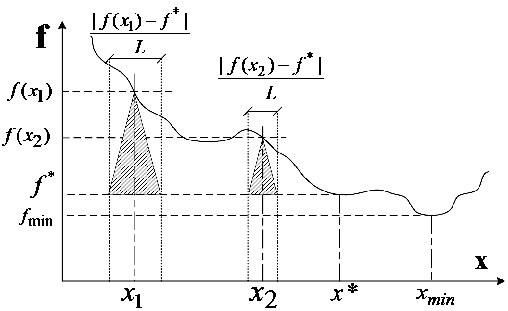
\includegraphics[width= \textwidth, height = 8cm]{Lipschitz-constant.png}
	\caption{A Lipschitz function with Lipschitz Constant L. $f*$ is the minimal value achieved so far. By evaluating the function at a single point $x$, a neighbourhood region with radius $\dfrac{|f(x) − f*|}{L}$ can be eliminated without losing the true global minimum $x \min$~\cite{RGLipschitz}.}
	\label{fig:LipschitzConstant}
\end{figure}

